%`
%\nonstopmode
\hbadness=100000
\documentclass[a4paper, 12pt]{article}
\usepackage{amsmath,amsfonts,caption,float,geometry,diagbox,graphicx,mathtools,pythonhighlight,textcomp,makecell,url,verbatim,subcaption,tabularx, longtable, ulem, hyperref, tikz} %,parskip
\geometry{ a4paper, total={170mm,257mm}, left=20mm, top=20mm}
\newcommand{\matr}[1]{\underline{\underline{\textbf{#1}}}}
\newcommand{\ve}[1]{\boldsymbol{#1}}
\newcommand{\Var}[1]{\text{Var}[#1]}
\newcommand{\apriori}{\textit{a priori}}
\newcommand{\chifit}{\frac{\chi^2_{fit\leftarrow meas}}{DoF} }
\newcommand{\chitrue}{\frac{\chi^2_{true\leftarrow meas}}{DoF}}
\newcommand{\pythoncode}[2]{
\DeclareMathOperator*{\argmax}{arg\,max}
\DeclareMathOperator*{\argmin}{arg\,min}
\begin{adjustwidth}{-1.3cm}{-1.3cm}
\texttt{#1}
\inputpython{#2}{1}{1500}
\end{adjustwidth}
}
\usepackage[toc, page]{appendix}
% \usepackage[dvipsnames]{xcolor}
% \definecolor{subr}{rgb}{0.8, 0.33, 0.0}
% \definecolor{func}{rgb}{0.76, 0.6, 0.42}

\begin{document}
\centering
% \includegraphics[width=8cm]{CoverPage/UoBlogo.pdf}
% \hrule
% \bigbreak
% \textbf{F}usion Neutron \textbf{Acti}vation Spectra \textbf{U}nfolding by \textbf{N}eural \textbf{N}etworks \\
% (FACTIUNN)                                      \\
% \hrule
% \bigbreak
% \begin{minipage}[b]{0.4\textwidth}
%     \includegraphics[height=2cm]{CoverPage/CCFElogo.jpeg}
%   \end{minipage}
%   \hfill
%   \begin{minipage}[b]{0.4\textwidth}
%     \includegraphics[height=3cm]{CoverPage/UKAEAlogo.jpeg}
% \end{minipage}
    
\begin{table}[!h]
\centering
\begin{tabular}{rl}
author:&Ocean Wong          \\
       &(Hoi Yeung Wong)    \\
supervisor:&Dr Chantal Nobs    \\
           &Dr Robin Smith     \\
advisor:&Prof Alison Bruce\\
date:  &May 2020       \\
Organization:&Culham Centre for Fusion Energy\\
            & Sheffield Hallam University
\end{tabular}
\end{table}
\hrule
\abstract
    This document attempts to explain why $\frac{\chi^2}{DoF} = 1$ should not be used in case of underdetermined unfolding/fitting; and instead $\chi^2=0$ should be used.
% \emph{Keywords:} Underdetermined unfolding
% \hline
% \twocolumn
% \tableofcontents
% \listoffigures
% \pagebreak
\begin{center}
\large{\chapter{The dangers of applying $\chi^2=1$ blindly}}\\
% \large{Also known as ``That one time when my statistics training comes in handy"}
\end{center}
\section{Introduction}
In physics we are hard-wired to use $\chi^2=1$ as a test of goodness-of-fit. But I warn that this is a dangerous practice to carry into the realm of underdetermined fitting.

This documents will approach in two ways. Section\ref{Intuitive section} will explain it in plain language with the aids of diagram, leveraging on only intuitive understandings of physics; while section \ref{Formal section} requires some familiarity with the $\chi^2$ distribution function.

\section{Intuitive Explanation}\label{Intuitive section}

Let's begin with the first use case that comes to a physicist's mind when $\chi^2$ is mentioned: linear regression.
\begin{figure}[H]
\centering
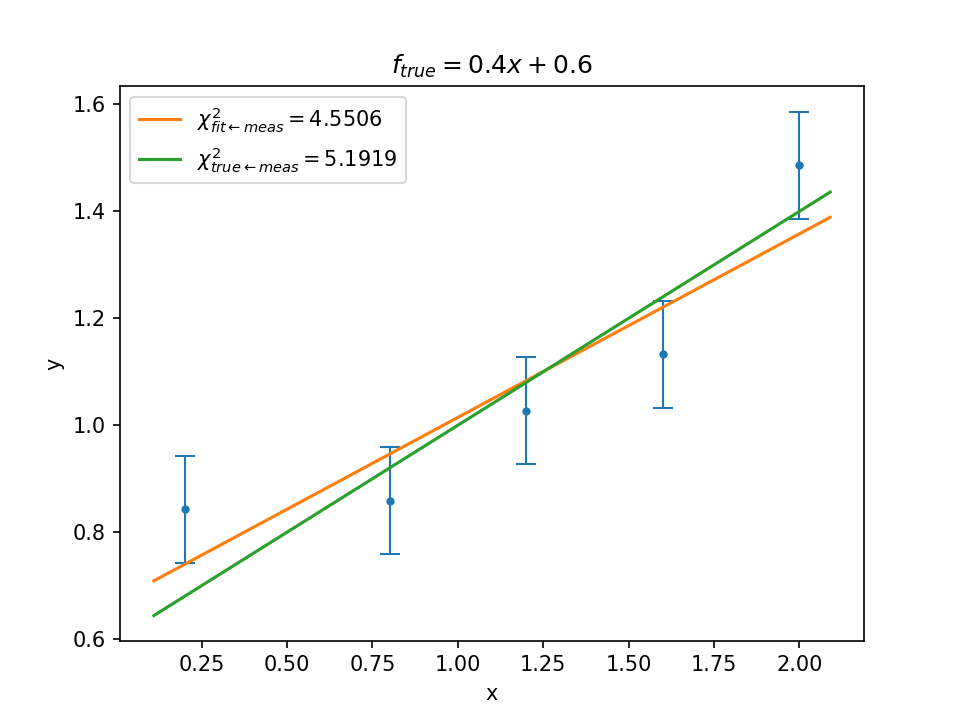
\includegraphics[width=0.5\textwidth]{A_linregress.png}
\caption{An example of linear regression. The underlying function used is $f_{true}=0.4x+0.6$.
% Five measurements were made to obtain samples at five different values of $x$, and a striaght line is fitted through it.
}\label{A_linregress}
\end{figure}

Let's say the measurements at $x$ is generated by a true function and some error,
\begin{equation}
    y(x) = f_{true}(x) + \sigma_{true}(x)
\end{equation}
where $\sigma_{true}$ is a non-deterministic function: its values, after being sampled many times, is Gaussian-ly distributed. $f_{true}$ is deterministic.

By the Law of Large Numbers, when many measurements are taken to obtain a mean, 
\begin{equation}
    <y(x)> = f_{true}(x)
\end{equation}

But if only one measurement is taken then one would expect $|y(x)-f_{true}(x)|^2 \approx \sigma^2_{true}(x)$ on average. Sometimes this deviation is overshoots the variance, and sometimes it undershoots.
\begin{equation}\label{on average equal 1 equation}
    \frac{|y(x)-f_{true}(x)|^2}{\sigma^2_{true}(x)}=1 \text{  on average}
\end{equation}

So if we make only one measurement at $x_1$, one at $x_2$, one at $x_3$, ... $x_N$, then we have
\begin{equation}\label{sum equal 1 true}
    \sum_i^N \frac{|y(x_i)-f_{true}(x_i)|^2}{\sigma^2_{true}(x_i)}=N
\end{equation}
If N measurements were made. 

(Don't get too complacent yet, this is NOT the typical chi-squared that we're used to seeing/talking about.)
L.H.S. of equation \ref{sum equal 1 true} is a measure of how far the measurement deviates from the true distribution. So let's label this quantity, divided by the number of measurements, as $\chitrue$
\begin{equation}\label{chi2true definition}
\chitrue = \frac{\sum_i \frac{|y(x_i)-f_{true}(x_i)|^2}{\sigma^2_{true}(x_i)}}{N}
\end{equation}
At this stage, as experimentalists, we don't have any knowledge of $f_{true}$. So unless you have an all-knowing God/deity by your side, who knows both $f_{true}$ and $\sigma_{true}$, you won't be able to know the value of $\chitrue$. (But if such a deity exist and is generous enough to do so, then he can calculate $\chitrue$ for you using equation \ref{chi2true definition}.)

But unfortunately (to the best of physics' knowledge) such a deity does not exist (or if they did, is a selfish one and won't share $f_{true}$ and $\sigma_{true}$ with us). Therefore we have to use some other methods than divination to infer $f_{true}$.

We can construct a function $f_{fit}$ over the same domain as $f_{true}$'s, to approximate $f_{true}$. (Orange line in Figure~\ref{A_linregress})

But how do we know if this $f_{fit}$ is a good approximation of $f_{true}$?

I mentioned $\chitrue \approx 1$ on average. If we can, somehow, define an analogous quantity to $\chitrue \approx 1$ for $f_{fit}$, and if this quantity $=1$, then we can say that $f_{fit}$ \textit{might} be a good fit. 

Let's call this analogous quantity $\chifit$. We can't define $$\chifit = \sum_i \frac{|f_{fit}(x_i) - y(x_i)|^2}{\sigma_{true}^2(x_i)}$$ because we still don't know what is $\sigma_{true}(x)$. We have to find a function to replace it.

So instead we use 
\begin{equation}\label{chi2meas definition}
    \chifit = \sum_i \frac{|f_{fit}(x_i) - y(x_i)|^2} {\sigma_{meas}^2(x_i)} ,
\end{equation}
where $\sigma_{meas}$ is a thing.

Now \textit{this} is the chi-squared format that everyone is used to seeing/talking about.

We can make multiple measurements at $x_i$ to get multiple values of $y$ as $y(x_i)_1, y(x_i)_2, y(x_1)_3, ...$, and calculate the variance of them $\Var{y(x_i)_1, y(x_i)_2, y(x_1)_3, ...}$, to be used in place of $\sigma_{true}^2(x_i)$. And then we can plug in $y(x_i) = y(x_i)_1$, $\sigma_{meas}=\Var{y(x_i)_1, y(x_i)_2, y(x_1)_3, ...}$ into equation\ref{chi2meas definition} to obtain $\chifit$.
\footnote{This is only a half-truth, written in place of the truth for simplicity. In reality, having made more measurements = obtained more information about the system; it would be foolish to let these new information go to waste. So instead we would plug in $y(x_i)=\overline{y(x_i)}=\frac{\sum\limits_j^M y(x_i)_j}{M}$ if M measurements were made, and $\sigma_{meas}^2(x_i)=\frac{\Var{y(x_i)_1, y(x_i)_2, y(x_1)_3, ...}}{M}$.}
Or, we can apply certain assumptions, such as assuming $f_{true}(x)+\sigma_{true}(x)$ follows a Poisson distribution, with mean $\lambda=f_{true}$.
\footnote{Poisson statistics allows us to infer the error $\sigma$ directly from a single measurement. Let's say we only measure for 1 minute y counts. Then the counts per minute has an error $\sigma_{meas}=\sqrt{y}$.}

\subsection{A graphical analogy}\label{Graphical proof}
The usual procedure of function fitting is as follows:
\begin{enumerate}
    \item Acquire measurements ($y(x_i)$ for a list of i=1, 2, ...)
    \item Propose a function, which usually may contain free parameters. e.g. $f_{fit}(m,c) =mx+c$ \label{propose function and fit}
    \begin{itemize}
        \item (If free parameters are present) fit them the best of your (/your computer's) ability by minimizing the root-sum-squared residuals through adjusting these free parameters. (e.g. via adjusting $m$ and $c$)
    \end{itemize}
    \item The optimized $f_{fit}$ is then expected to have $\chifit\approx 1$ \label{goodness of fit test point}
\end{enumerate}

Step \ref{propose function and fit} has the effect of descending down the negative-log-likelihood surface.

\begin{figure}[H]
\centering
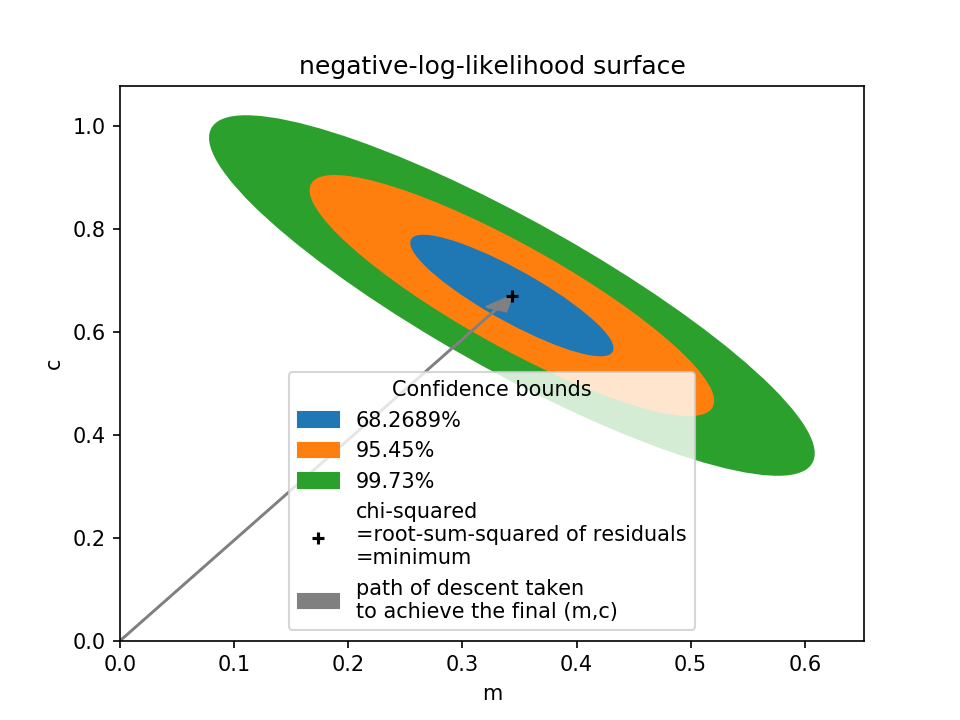
\includegraphics[width=0.7\textwidth]{Phase_space.png}
\caption{The phase space of the fitting parameters used in figure \ref{A_linregress}. Each point on this graph corresponds to a combination of (m,c) that gives a $f_{fit}=mx+c$. Thus we can calculate a value of $\chifit$ for each point on this graph.
For Gaussian distributions, the chi-square function $=2\times$ negative log likelihood function. The edges of the concentric ellipses are equivalent to the contour lines encircling the centre of the chi-squared surface bowl.
}\label{Phase_space}
\end{figure}

After that, the goodness-of-fit test performed in step \ref{goodness of fit test point} gives a positive result(i.e. $f_{fit}=f_{true}$) if $\chifit=1$, vice versa. 

It so happens that, in this particular fit, $\chifit=\frac{5.1919}{5}\approx 1$, passing the goodness-of-fit test.

Graphically speaking, the black cross in figure \ref{Phase_space} (at the bottom of the bowl) is expected to have $\chifit=1$. Otherwise, we may have a function $f_{fit}\neq f_{true}$.

However, in the underdetermined case, the $\chi^2$ surface is quite different: It has at least one singular direction, i.e. a direction along which the negative-log-likelihood function does not vary, and there is always some points where $\chifit$ can equal 0.

\begin{table}[H]
\begin{tabularx}{\textwidth}{|X|X|X|}
\hline
Source of the program & Relies on simultaneously minimizing distance to the $\apriori$ and $\chifit$ of radionuclide populations (error propagation possible) & Change the spectrum iteratively, starting from the a priori (error propagation not possible)\\
\Xhline{2\arrayrulewidth}
\href{https://www.oecd-nea.org/tools/abstract/detail/nea-1665}{UMG3.3}& \href{https://doi.org/10.1097/00004032-199911000-00012}{MAXED}: extremize cross-entropy (in a weird form that I do not agree with) while keeping $\chifit$ at a user-defined value. Can be trapped in sub-optimal points. & \href{http://matzke-bs.de/heprow/Dateien/HEPROW.PDF}{GRAVEL}\\
\hline
Improved from UMG 3.3 (by me)& \href{https://ukaeauk-my.sharepoint.com/:b:/g/personal/chantal_nobs_ukaea_uk/EbLCFG4TD_NJkPLoaduueGgBtVJqSfxOZLLn5zvsWGRkCA?e=31ufjm}{IMAXED}: maximizes the same quantity as above, but uses a different optimization algorithm so it converges faster, and gives higher quality results. (Gets much closer to the maximum point than MAXED can ever dream of achieving)
 & \\
\hline
My own invention& \href{https://ukaeauk-my.sharepoint.com/:b:/g/personal/chantal_nobs_ukaea_uk/Ee3pm8efH11BvZsbbeR7umkBfwP77h5v8KbnyaWB1JeSgw}{Regularization code}: extremize the cross-entropy in the correct form& Pseudo-inverse (documentation pending): Apply pseudo-inverse to approach the solution spectrum\\
\hline
\end{tabularx}
\caption{Categories of unfolding algorithms, and some prominent examples for each categories}\label{Unfolding algorithms category table}
\end{table}
Unfolding algorithms can be broadly divided into one of three categories. The first two are listed at the top of column 2 (minimize distance from \apriori) and 3 (start from \apriori, take steps until $\chifit<$threshold) of Table \ref{Unfolding algorithms category table}. The third kind is parametrisation, i.e. assume the neutron spectrum is a combination of Maxwellian and Watt distribution, reduces the dimensionality of the problem to avoid the problem of underdetermination altogether. However, this dimensionality reduction approach is not mature enough to be applied in Fusion Neutron physics, thus is not discussed here.

Limited by the number of dimension of the medium that I'm presenting through, I can only show an underdetermined system with two neutron bins and one type of radionuclide population ($n=2, m=1$). (See appendix\ref{Prologue} for a refresher on the terms used.)

Let's say we have\\a response matrix (shape = $m \times n$) \matr{R} = 
$
\begin{pmatrix}
1 & 2
\end{pmatrix}
$, \\
a true spectrum $\ve{\phi_{true}}=(1,2)$;\\
then the true radionuclide populations is $\ve{N_{true}}=\matr{R}\ve{\phi_{true}}=5$,
and $\sigma_{true}=\sqrt{5}$.\\
And let's say our $\apriori$ is somewhere in the vicinity of the true spectrum, $\ve{\phi_{ap}}=(1.25, 2.6)$.
(The usual units apply.)\\

This means that if this experiment is repeated many times, the experimenters will find on average $\ve{N}=5$, with a standard deviation $\sigma(\ve{N})=\sqrt{5}$.

But unfortunately neutron spectrum measurement experiments are expensive and resource intensive, so it is likely that we will only have one measurement. Let's say in our first experiment, $\ve{N_{meas}}=6$. Then we will assume $\sigma=\sqrt{6}$.

% a measured radionuclide population $\ve{N}=8\pm1$.\\
The response matrix spans $m=1$ dimension, while leaving the remaining $n-m=1$ direction undetermined (singular).

Since the response matrix spans the $\frac{1}{\sqrt{1^2+2^2}}(1,2)$ direction, the singular direction is the direction orthogonal to that, i.e. $\frac{1}{\sqrt{1^2+2^2}} (-2,1)$.

\begin{figure}[H]
\centering
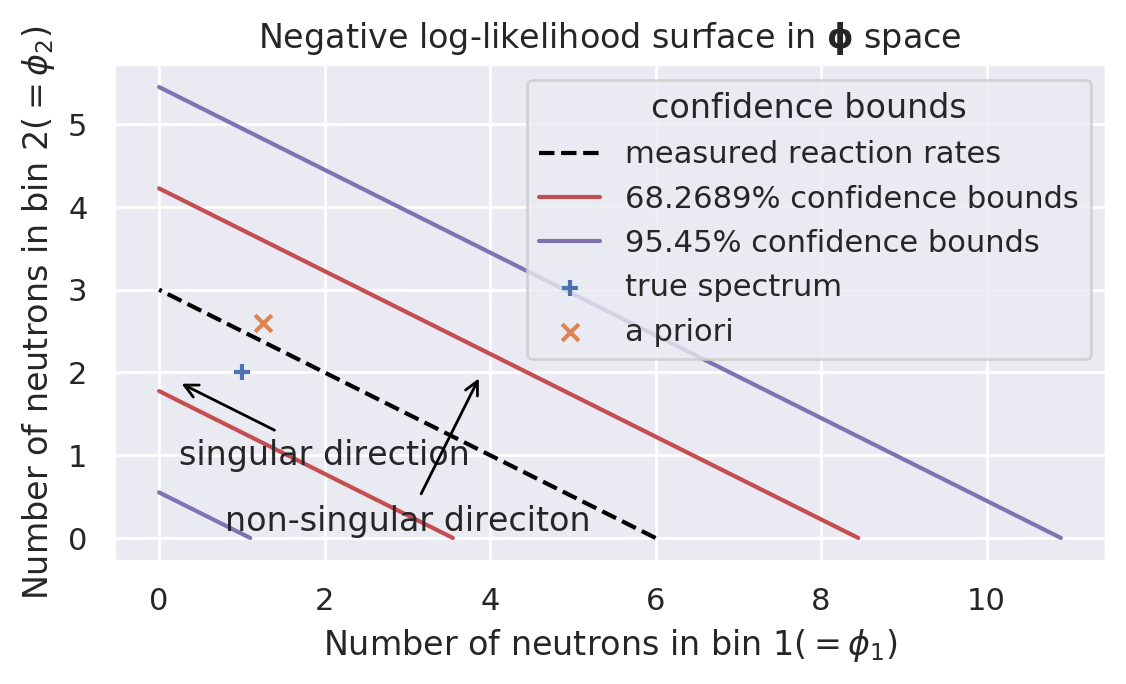
\includegraphics[width=0.7\textwidth]{Singular_log_likelihood.png}
\caption{The negative log likelihood function in an underdetermined system must have at least one singular direction, and there must be more than 1 point corresponding to $\chifit=0$ (Denoted with the dotted line here.)}\label{Singular_log_likelihood}
\end{figure}

Notice that all contour lines are aligned in the singular directions. This is because, in an underdetermined system, any changes in $\ve{\phi}$ along the singular direction(s) will not affect the outputted radionuclide populations. In other words these contour lines are also ``iso-radionuclide-population" lines.
Any $\ve{\phi_{test}}$ on the same line will produce the same set of radionuclide population(s).
% It doesn't matter where along this line  $\ve{\phi_{true}}$ is, it will not be noticed by the experimenter.

Thus the $\chi^2$ surface forms a parabolic ``trench" instead of the familiar bowl shape in figure \ref{Phase_space}.
    
By examining figure \ref{MAXED path of descent} and \ref{GRAVEL path of descent}, it becomes intuitive why setting $\chifit$ is an incorrect practice.

Bearing in mind that our goal is to find a solution $\ve{\phi_{sol}}$ as close to $\ve{\phi_{true}}$ as possible, setting $\chifit=1$ gives a solution worse than setting $\chifit=0$.

\begin{figure}[H]
\centering
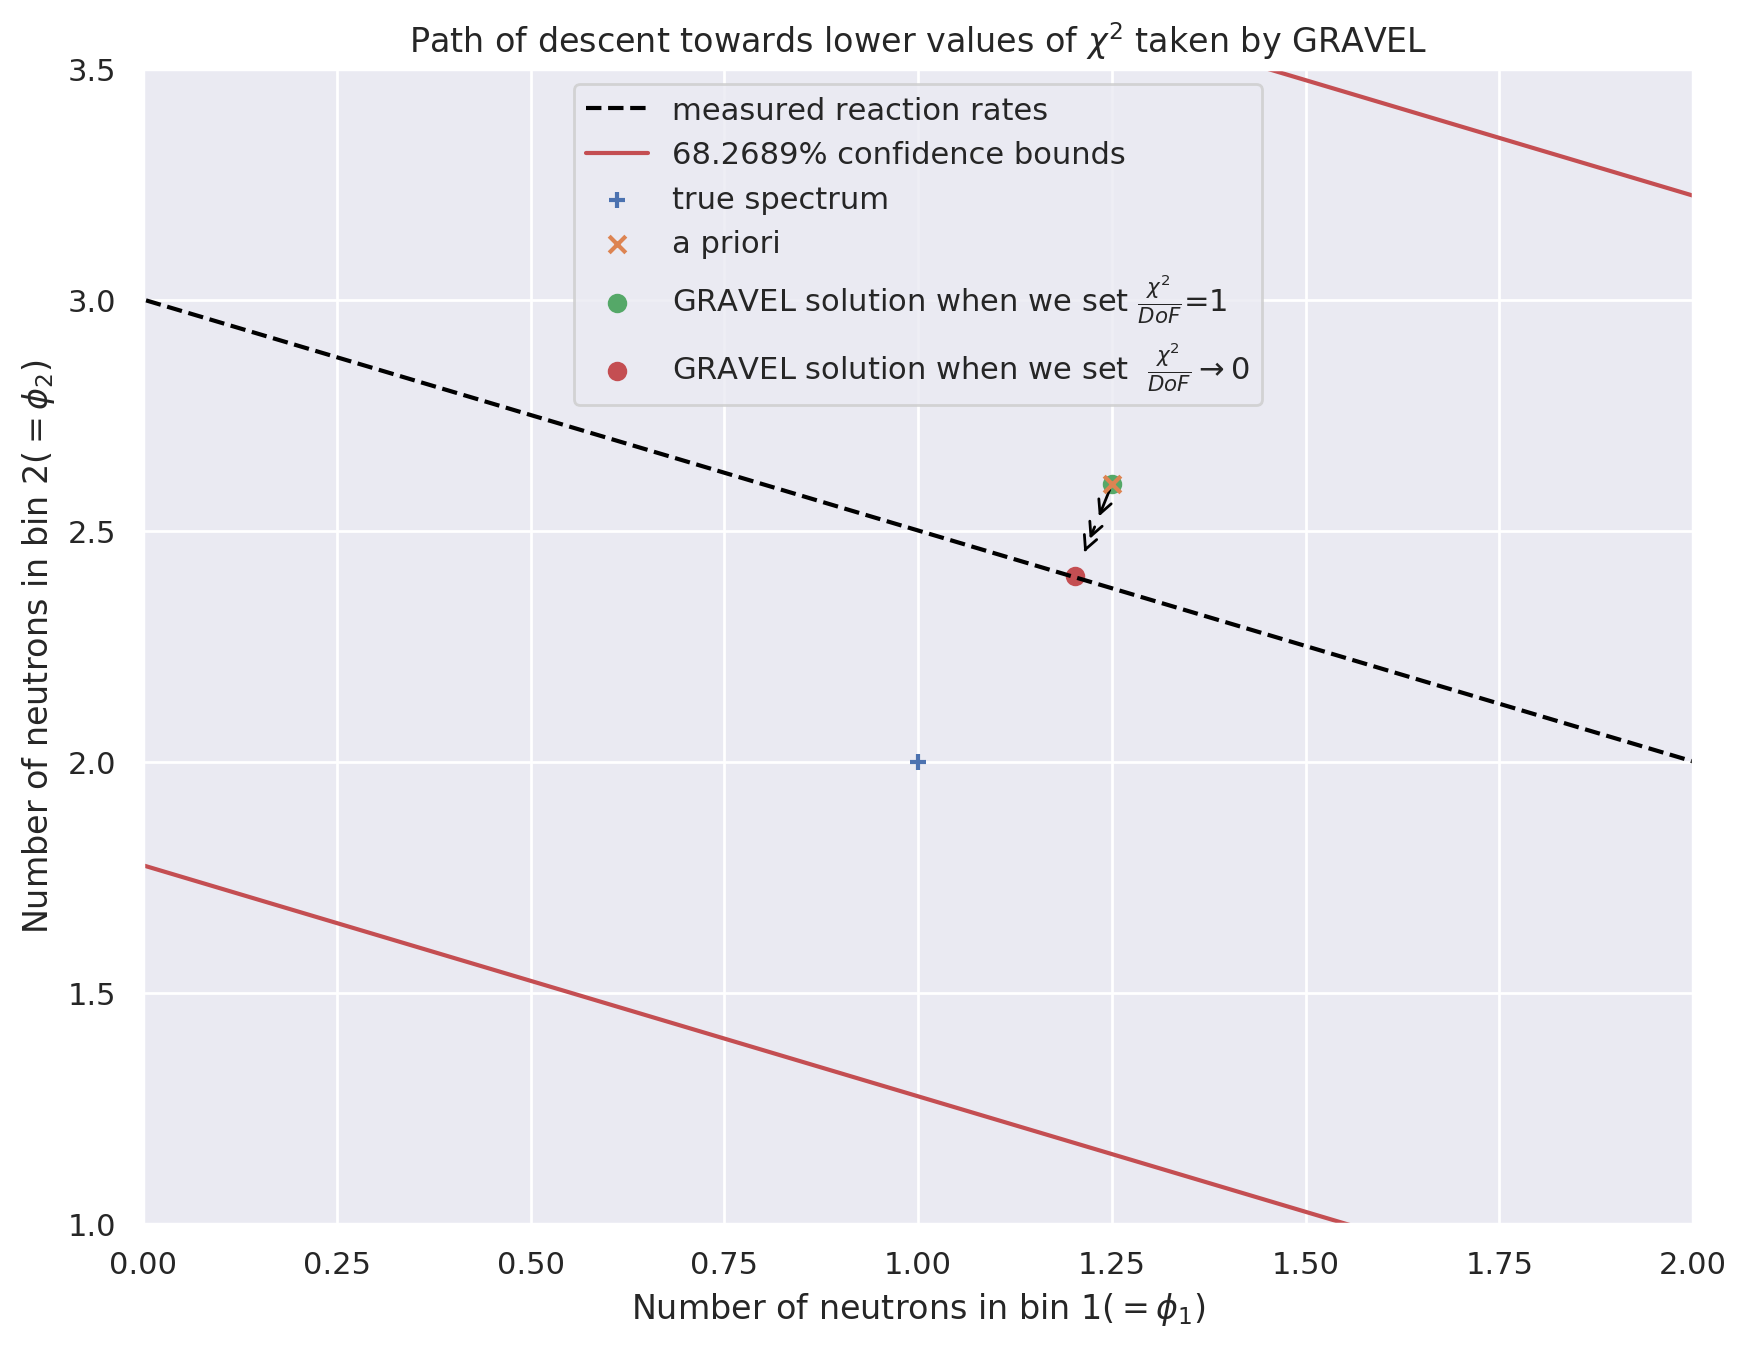
\includegraphics[width=\textwidth]{GRAVEL_descent.png}
\caption{The solutions that GRAVEL will output when different termination values of $\chifit$ is inputted. Note that in the first case, the $\apriori$ was outputted directly, as the solution started in a place where $\chifit<$termination value=1.
(In figure \ref{Singular_log_likelihood}, $\chifit<1$ within the red lines, $\chifit<4$ within the purple lines.)
}\label{GRAVEL path of descent}
\end{figure}
GRAVEL takes steps towards the centre-line of the trench, monitoring the $\chifit$ after each step, and terminates when $\chifit$ drops below a user-defined value.
\begin{figure}[H]
\centering
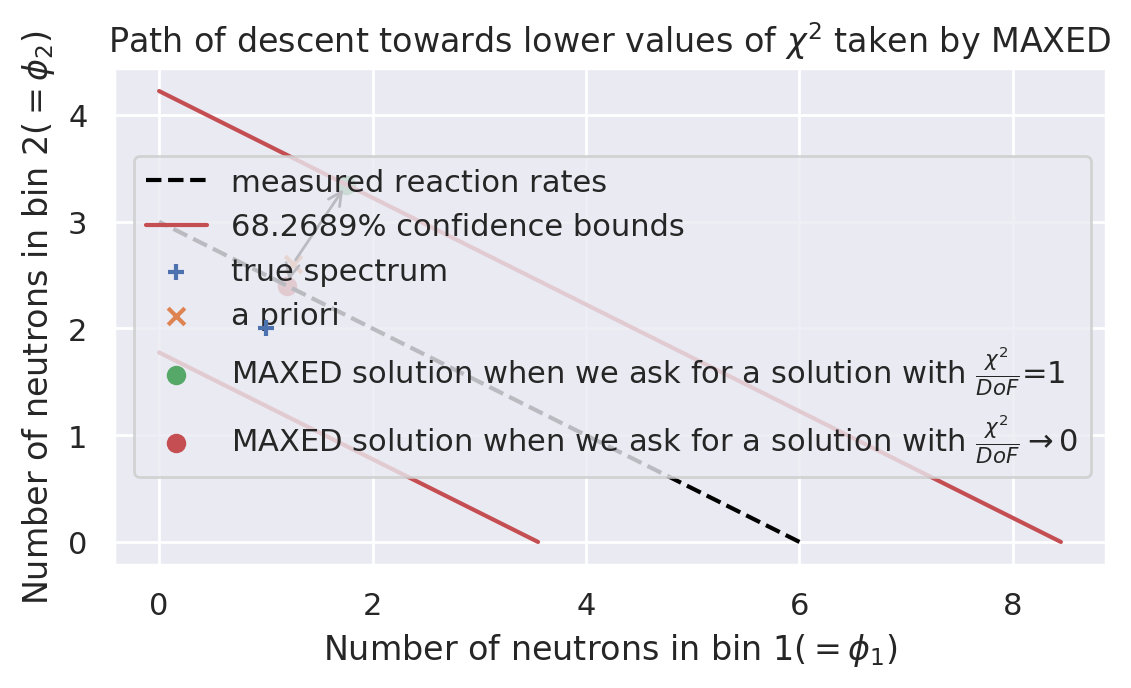
\includegraphics[width=0.8\textwidth]{MAXED_descent.png}
\caption{The solutions that MAXED will output when using different input of ``desired $\chifit$"}\label{MAXED path of descent}
\end{figure}
MAXED uses the value of $\chifit$ inputted by the user as part of its constraint, and extremize the cross-entropy between the solution spectrum and the $\apriori$ spectrum.

To make this argument more convincing, I can repeat the process above in a Monte Carlo approach: while keeping both the $\apriori$ and the $\phi_{true}$ fixed, simulated measurements of the radionuclide populations $\ve{N}$ can be generated via the non-deterministic function $\ve{N_{true}} + \sigma_{true}(\ve{N})$, and the unfolded solution can be plotted as a dot. We will then generate two collections of dots for each algorithm, one for the $\chifit=1$ solutions for each algorithm, and one for the $\chifit\rightarrow0$ solutions for each algorithm. We can then see that the $\chifit=1$ cloud of dots is spread further away from $\ve{\phi_{true}}$.

However, this exercise is rather time-consuming and does not convincingly prove that the same holds in higher dimensions. Therefore I have opted to not make such a graph.

% \section{Additional evidence}\label{Formal section}
\section{The relationship between chi-squared (the quantity), and chi-squared (the distribution)}\label{Formal section}
    % \subsection{The validity of the $\chi^2$ goodness of fit test}\label{Confusion matrix section}
    % Another point to note is that, the goodness-of-fit test performed in step \ref{goodness of fit test point} is only a vastly simplified way of testing for what we actually want to know (if $f_{fit}=f_{true}$).
    % % Therefore it can be prone to error and stuff.
    % \begin{table}[H]
    % \centering

    % \begin{tabularx}{0.8\textwidth}{|X|X|X|}
    % \hline
    % % \backslashbox{Goodness of fit test result}{True result} & $f_{fit}=f_{true}$ & $f_{fit}\neq f_{true}$\\
    % \makecell{Goodness of fit\\test result} & $f_{fit}=f_{true}$ & $f_{fit}\neq f_{true}$\\
    % \hline
    % \makecell{Passed\\($\chifit\approx1$)} &
    % \begin{enumerate}
    %     \item $f_{fit}=f_{true}$ and $\chitrue\approx1$
    % \end{enumerate}
    % &
    % \begin{enumerate}
    %     \setcounter{enumi}{1}
    %     \item Coincidence: wrong type of function used as $f_{fit}$, but still worked
    %     \item Coincidence: The measurements happens to line up in a different trend than $f_{true}$.
    %     % Measurements happens to be laid out in such a way that the minimum achievable $\chifit=1$: Improbable ($\chitrue$ very high).
    %     % Wrong class of function used, but somehow also got a good fit.
    % \end{enumerate}
    % \\
    % \hline
    % \makecell{Failed\\($\chifit\neq1$)} &
    % \begin{enumerate}
    %     \setcounter{enumi}{3}
    %     \item Coincidence: $\chitrue\neq1$ to begin with
    %     \item Over-/under-estimation of $\sigma_{meas}$\label{over-under-estimation1}
    % \end{enumerate}
    % &
    % \begin{enumerate}
    %     \setcounter{enumi}{5}
    %     \item Wrong type of function used
    %     \item Over-/under-estimation of $\sigma_{meas}$\label{over-under-estimation2}
    % \end{enumerate}
    % \\
    % \hline
    % \end{tabularx}
    % \caption{The confusion matrix for the chi-squared goodness of fit test in fully-determined systems, and some plausible circumstances for each corner of the matrix.} \label{Confusion matrix}
    % \end{table}
    % % Insdert examples for each except for the repeated \ref{over-under-estimation1} case.
    % % Let's say that we are good experimentalist and did not end up in situation \ref{over-under-estimation1} or \ref{over-under-estimation2}.

This whole time we have been discussing the reduced-chi-squared $=\chifit \approx 1$ if we're not unlucky.
% (i.e. we didn't incidentally fall into the top right/bottom left corner of the confusion matrix (table \ref{Confusion matrix}))
However, I have not yet quantified how close to unity is `$\approx 1$'. This ambiguity will be resolved in the following section; along with it we will discover another piece of evidence, alluding to the fact that using $\chifit=1$ is wrong.

Each time we perform an experiment and perform a fitting procedure, we will obtain a slightly different set of measurements, and a slightly different value of $\chifit$. And although we can't know it, this set of measurements will also have a value of $\chitrue$.

Let's say we repeat the ``experiment" 16 times. Then we have a list of 16 $\chi_{fit\leftarrow meas}$ and 16 $\chi_{true\leftarrow meas}$.

\begin{figure}[H]
\centering
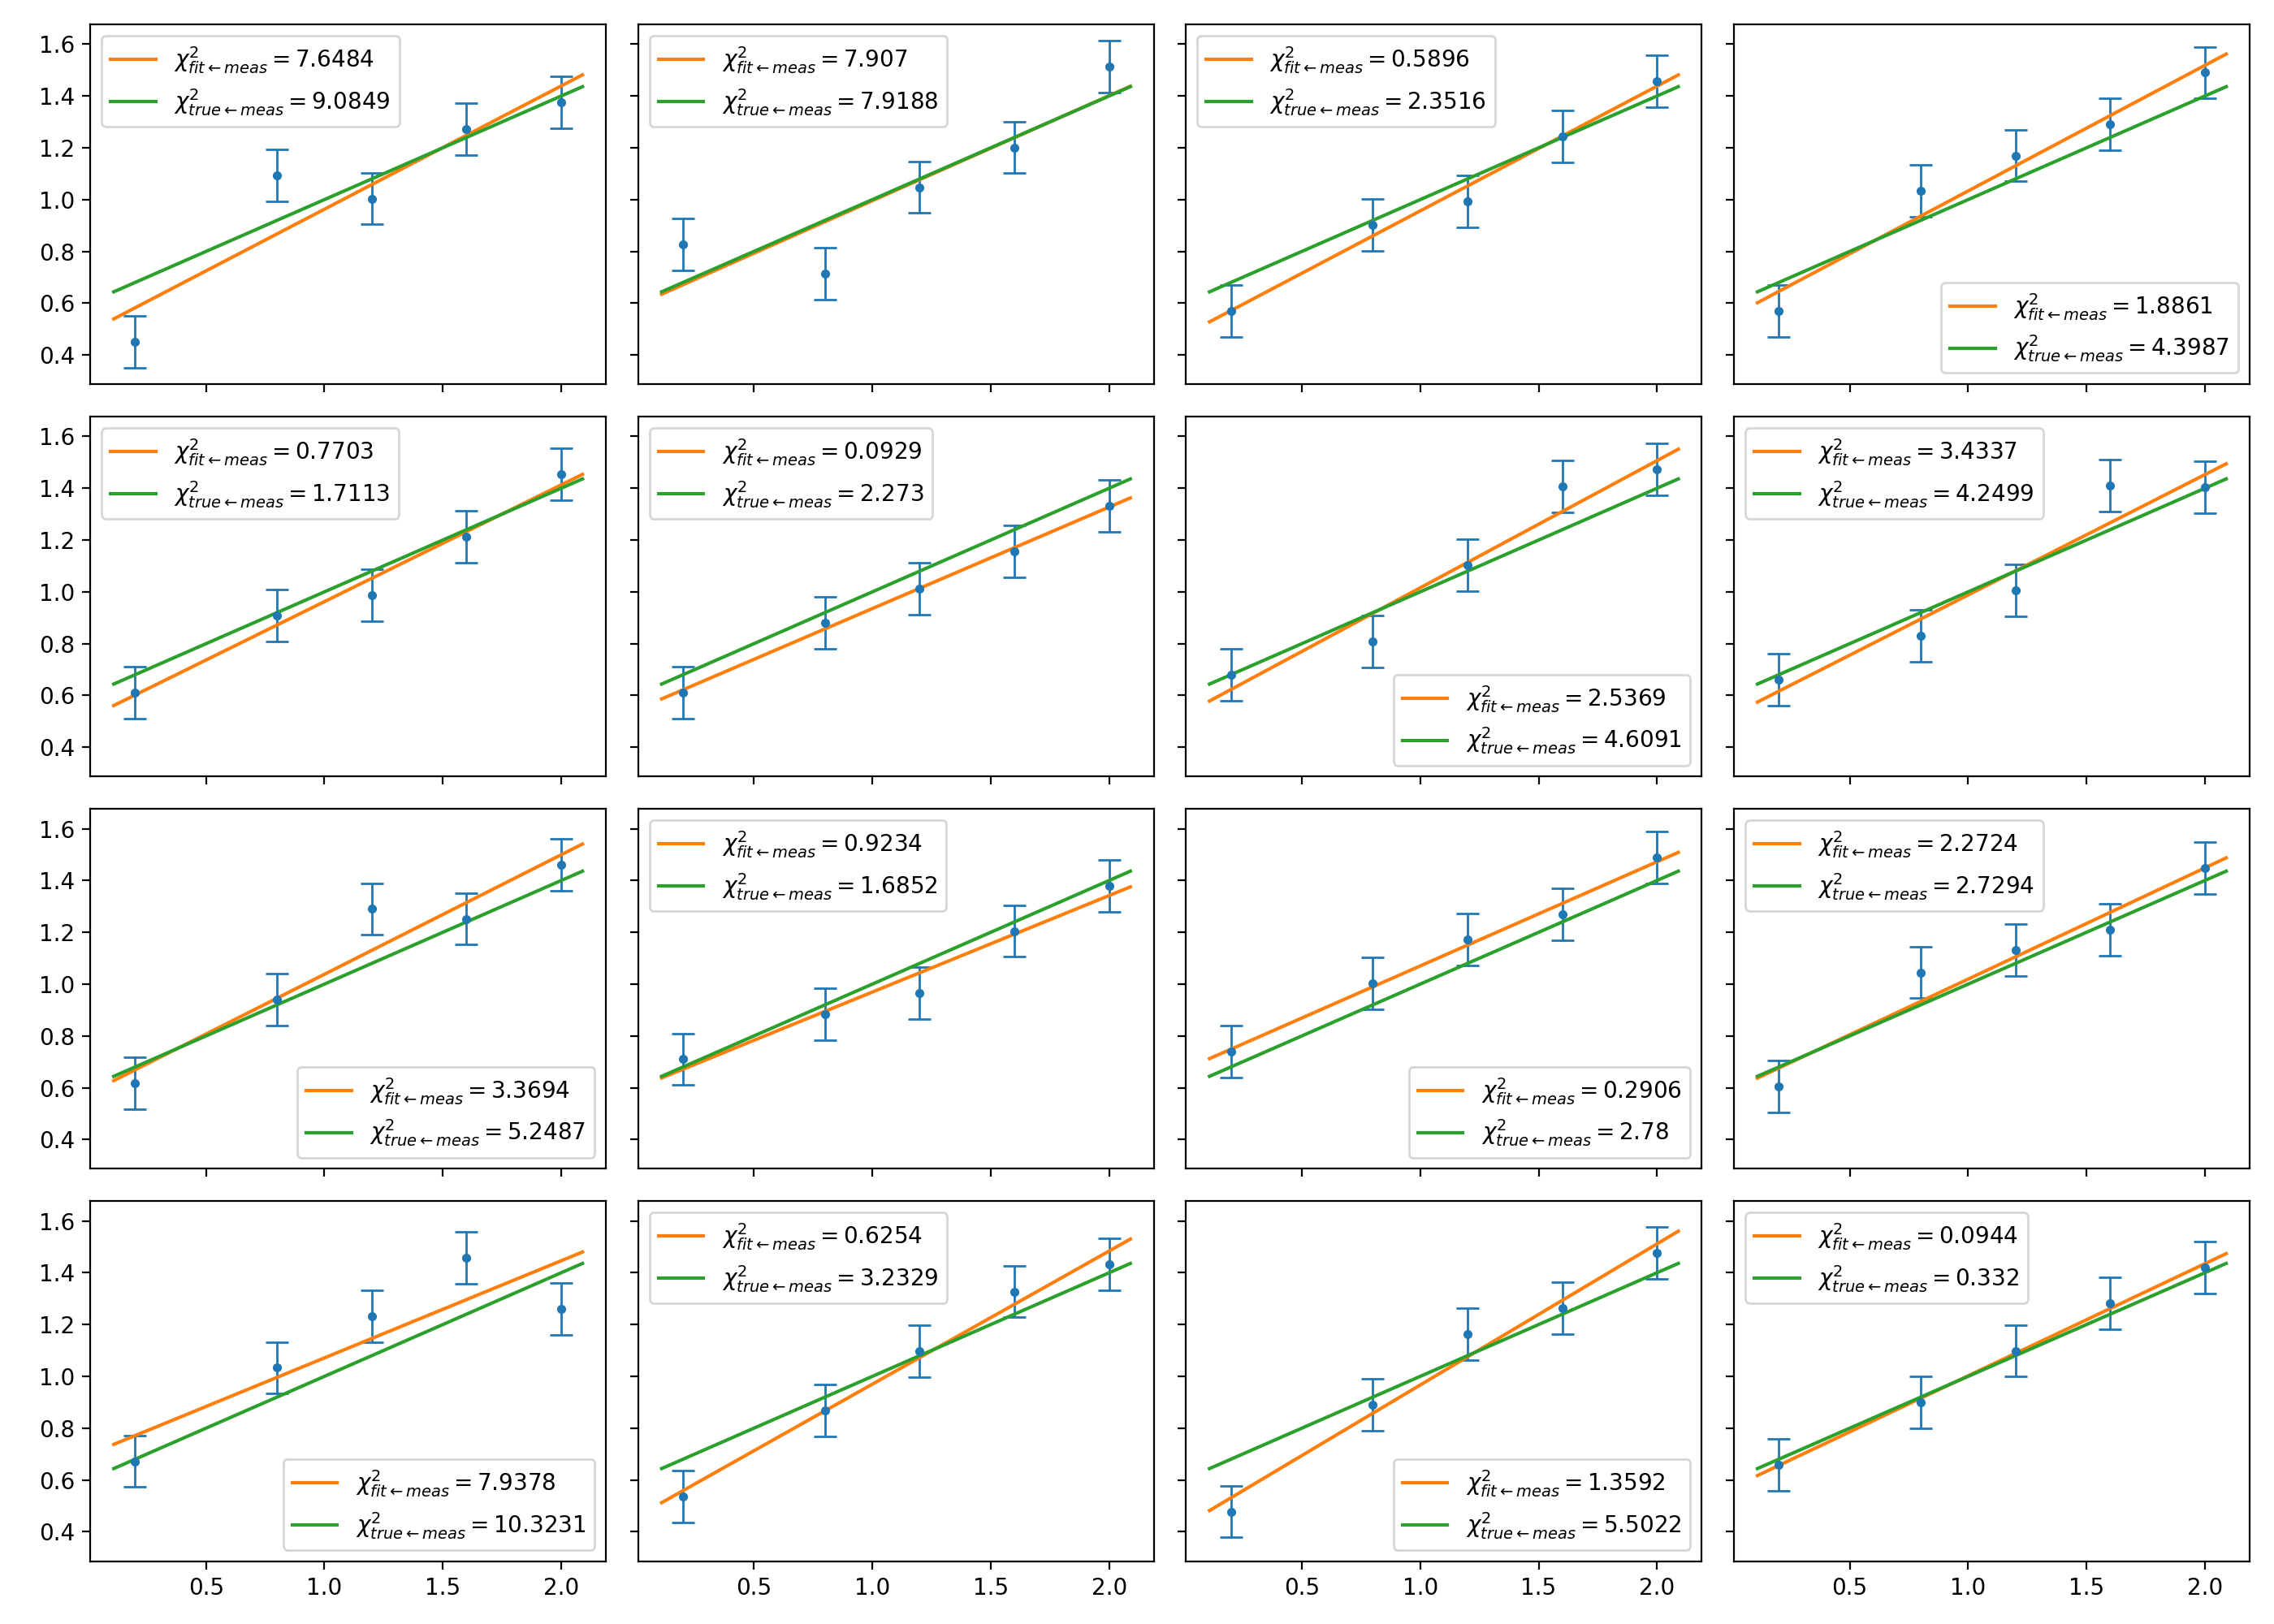
\includegraphics[width=1.1\textwidth]{Ensemble_of_linregress.png} %Stupid latex doesn't allow two dots in the filename.
\caption{Two distributions of $\chi^2$ values are obtained after 16 simulated experiments, each ``experiment" uses 5 data-points.} \label{Ensemble_of_linregress}
\end{figure}

Note that $\chifit$ is necessarily smaller than or equal to $\chitrue$ in each simulated experiment. This is because there may exist an $f_{fit}$ which fits the data better than $f_{true}$ (i.e. with a smaller value of root-sum-squared residuals). This is the first hint that $\chitrue$ and $\chifit$ should follow different distributions.

We can go even further and create 1000 of the graphs above, and plot the distribution of these $\chi^2$'s on a histogram.

\begin{figure}[H]
\centering
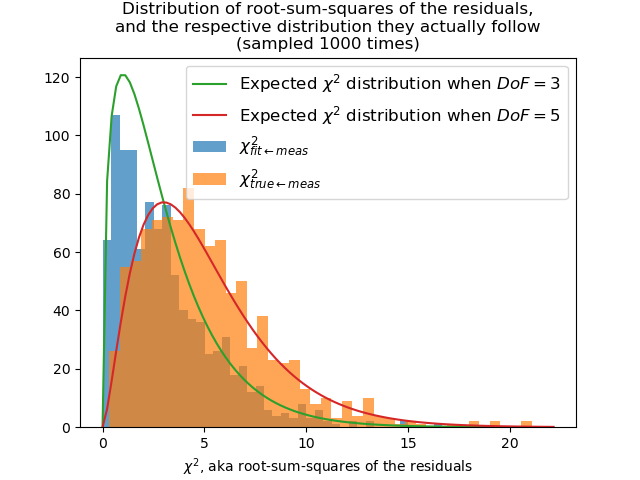
\includegraphics[width=0.6\textwidth]{Distribution_of_chi2.png}
\caption{Distribution of $\chi^2$ values in 1000 simulated experiments. 5 data points are generated per simulated experiment. Note that $\chifit$ and $\chitrue$ follows different distribution.}
\end{figure}

At this point it becomes clear how the probability distribution known as ``\href{https://en.wikipedia.org/wiki/Chi2_distribution}{$\chi^2$ distribution}" get its name. As we repeat simulated experiments and accumulate $\chi^2$'s values, they starts to follow respective $\chi^2$ distributions.

Since 5 measurements are taken per simulated experiment, $\chitrue$ follows the distribution of $\chi^2$ for 5 degrees of freedom. $\chifit$ is generated after fitting the five data-points to a function with two free parameters, reducing its DoF from five to three. Therefore it follows the $\chi^2$ distribution for 3 degrees of freedom.

The situation above is generated with over-determined system, i.e. more data-points than there are free parameters. But in case of underdetermined unfolding, we have more free parameters in the model than there are data-points.

\begin{figure}[H]
\centering
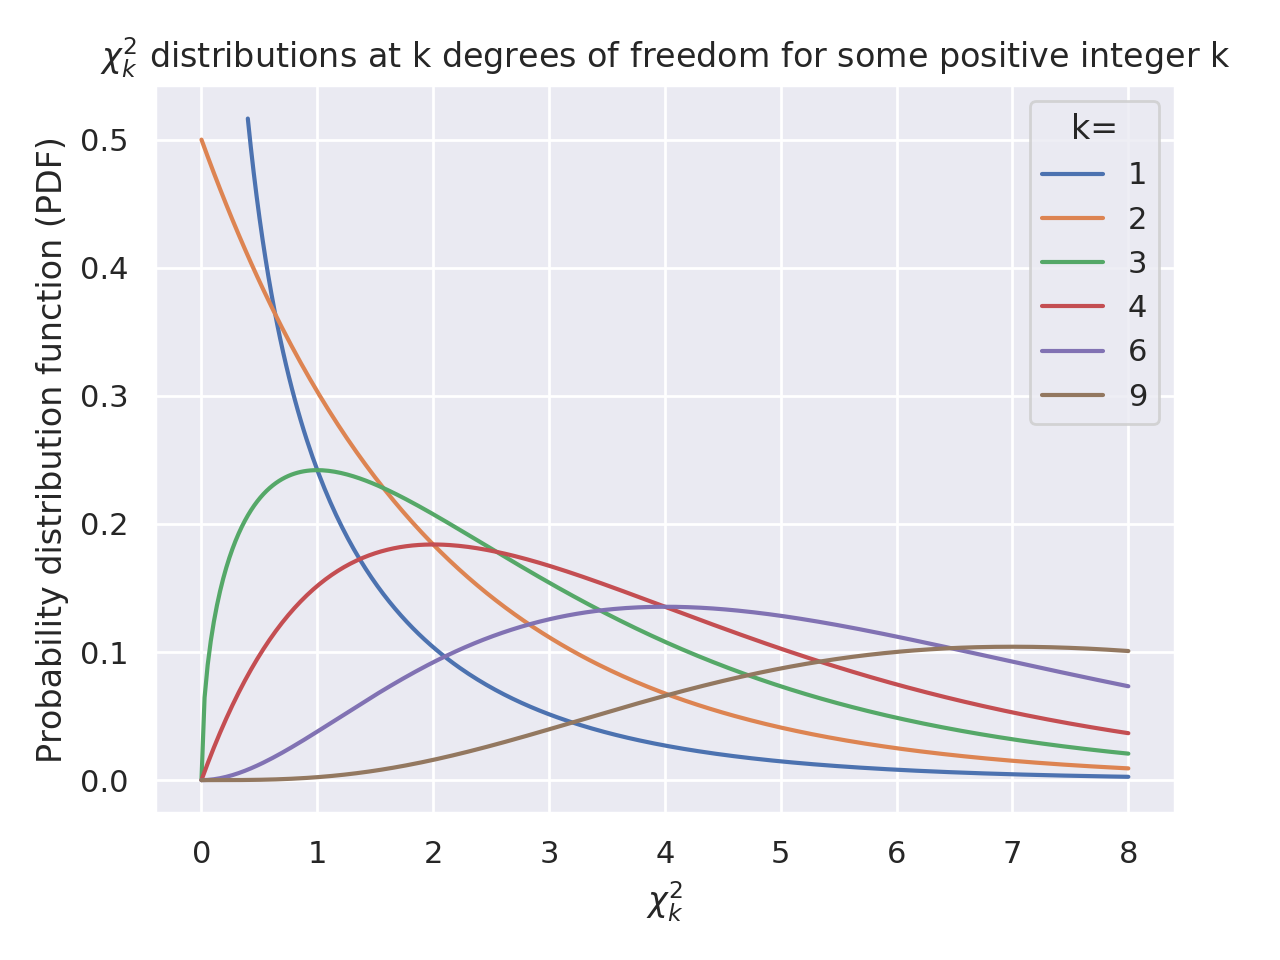
\includegraphics[width=0.6\textwidth]{Wiki_chi2.png}
\caption{The $\chi^2$ distributions at various positive degrees of freedoms.}\label{Wiki_chi2}
\end{figure}

\begin{figure}[H]
\centering
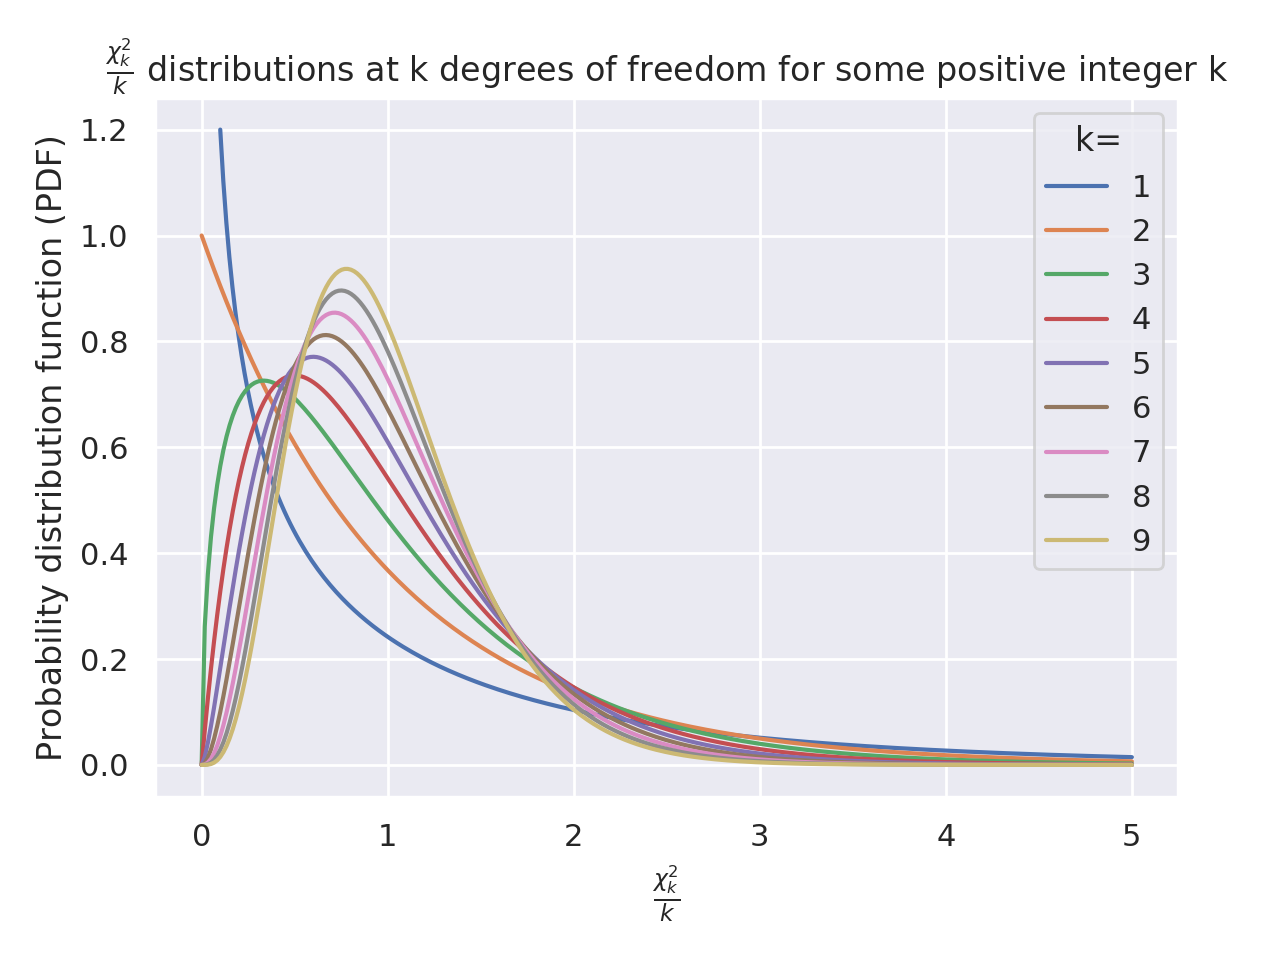
\includegraphics[width=0.7\textwidth]{Normalized_chi2_DoF.png}
\caption{The PDF of $\frac{\chi^2_k}{k}$ for various $k$. $k$ is used in place of DoF here. Note that both the denominator and the numerator are dependent on k.}\label{Normalized_chi2_DoF}
\end{figure}

For all positive integer values of k, the mean (first moment) of the $\chi^2_k$ distribution is $k$. This is the reason why we are usually told that $\chifit$ should equal 1. 

(For your information, the median of the $\chi^2$ distribution is $\approx k(1-\frac{2}{9k})^3$ and the mode is $max(k-2, 0)$. The variance $\sigma^2=2k$, therefore as k increase, the standard deviation from the mean of $\frac{\chi^2_k}{k}$ decreases as $\sigma(\chi^2)= \frac{2}{\sqrt{k}}$.)
% \cite

And as the number of degrees of freedoms increases, the $\frac{\chi^2_k}{k}$ distribution concentrates around 1. In other words, the more redundant measurement the experimenters makes, the more likely they will find their $\chifit\rightarrow1$, with decreasing likelihood to deviate from 1.

But knowing the behaviour of $\chifit\rightarrow1$ as $DoF\rightarrow\infty$ is not important to us. We want to know what happens when $DoF$ decreases, and eventually becomes negative as the number of free parameters exceeds the number of measurements.

% Unfortunately this is not possible as the $\chi^2_k$ distribution is undefined when $k\leq0$.
\begin{equation}\label{chi2 definition}
    \chi^2_k (x)=\frac{1}{2^{k/2} \Gamma \left( k/2 \right)}
                  x^{k/2-1} \exp \left( -x/2 \right)
\end{equation}
% \cite

We can use the equation above to infer what happens when $k\leq0$. As $k\rightarrow k'$ for any negative integer $k'$, $\frac{1}{\Gamma(k)}\rightarrow0$, thus $\chi^2_k(x)=0 \forall x\neq0$. Since we have defined $\chi^2_k$ to be a probability distribution, integrateing the area under its curve must give unity, i.e.$$\int_{x=0}^{x\rightarrow\infty}\chi^2_k(x)=1$$. Therefore, 

\begin{align}    
\chi^2_k(x)=\delta(x) & & \forall k \in\mathbb{Z}^{\leq0}
\end{align}

when k is a nonpositive integer, with mean, mode, median and variance all $=0$.

In other words, the expected $\chifit=1$ if $DoF>0$, else $\chifit=0$.

% Therefore with this approach we can only say that we don't have a meaningful expectation of $\chi^2_{fit\leftarrow meas}$; but we know that it must be smaller than $\chi^2_{true\leftarrow meas}$, usually by the number of free parameters in the model $n$. But since the value of $\chi^2$ must always be nonnegative, we can't say that the expectation value of $\chi^2_{fit\leftarrow meas}=m-n$ when $m<n$.

% We are then faced with the intractable problem of specifying a value of $\chi^2_{fit\leftarrow meas}$ for the MAXED and GRAVEL programs when there is no meaningful expectation value of the $\chi^2_{fit\leftarrow meas}$.
In light of this, I propose that we set $\chi^2_{fit\leftarrow meas}=max(m-n,0)$ for a dataset with $m$ data-points fitted to a model with $n$ degrees of freedoms, assuming that the model is correct.
Therefore we should set the value of $\chi^2_{fit\leftarrow meas}$ to a very small value for GRAVEL (since GRAVEL will never reach $\chi^2_{fit\leftarrow meas}=0$ with finite computing time) and set $\chi^2_{fit\leftarrow meas}=0$ for MAXED.
% I propose that we set the value of $\chi^2_{fit\leftarrow meas}$ to a very small value (since GRAVEL will never reach $\chi^2_{fit\leftarrow meas}=0$ with finite computing time, while MAXED will fail to perform its matrix inversion when $\chi^2_{fit\leftarrow meas}=0$).

% Can prove this by showing that using the n free parameters, the model can reach all possible states of m?

% \bibliographystyle{plain}
% \bibliography{FACTIUNN}
\section{Conclusion}
Previous users and creators of unfolding program MAXED and GRAVEL has the misconception that $\chifit$ = $\chitrue$ = $m$, which is incorrect. The degrees of freedom in $\chitrue$ = $m$ = number of data-points, while $\chifit$ = $m-n$ = number of data-points - number of free parameters adjustable by the fitting algorithm.

The expectation value of $\chi^2_{fit\leftarrow meas}=max(0, m-n)$, as shown in section \ref{Formal section}. Therefore in case of underdetermined unfolding when $m<n$, we should use $\chi^2_{fit\leftarrow meas}=0$.

% Applied to our underdetermined unfolding system, where the neutron flux (or fluence) in $n$ bins needs to be inferred from only $m$ measurements of radionuclide populations $\ve{N}$, and $m<n$, then we can say that we expect the $\chi^2_{true\leftarrow meas}=\sum\limits_j^m \left(\frac{N_{meas, j}-N_{true, j}}{\sigma_{true}(N_j)}\right)^2$ to be distributed as a $\chi^2$ distribution with $m$ degrees of freedom; while $\chi^2_{fit\leftarrow meas}=\sum\limits_i^m \left(\frac{N_{meas, j}-N_{fit,j}}{\sigma_{meas}(N_j)}\right)^2$ follows a $\chi^2$ distribution with $m-n$ degrees of freedom; but since it has an invalid number of degrees of freedom (negative), we can't say anything meaningful about the distribution of $\chifit$, or what we expect the value of $\chifit$ to be. %without making some assumptions about the measurement system.

% To solve this intractable problem, taking into consideration the results of section \ref{Intuitive section}, I propose $\chi^2_{fit\leftarrow meas}=max(m-n, 0)$.
% \pagebreak
\begin{appendices}
\section{Neutron spectrum unfolding}\label{Prologue}
Neutron spectrum unfolding using activation foils involves the following procedure:
\begin{figure}[H]
\centering
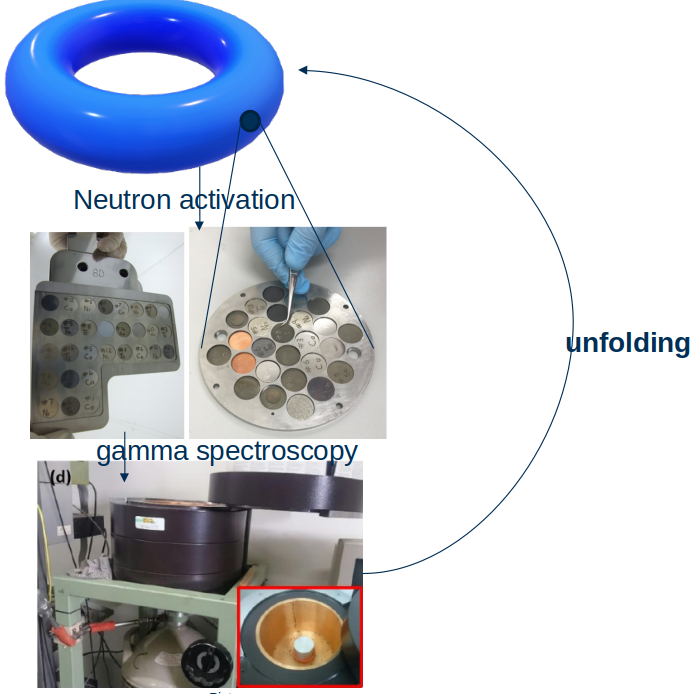
\includegraphics[width=8cm]{00_diagram.png}
\caption{Unfolding procedure}
\end{figure}
\begin{enumerate}
    \item Bathe a selection of foils in the unknown neutron spectrum, thus activating them;
    \item Extract them from the test environment;
    \item Measure the radionuclide populations inside each foil, by measuring the intensities of known gamma peaks;\label{measurement}
    \item Infer the neutron spectrum using an unfolding algorithm.\label{Algorithm}
\end{enumerate}

The algorithm in \ref{Algorithm} requires the following inputs:
\begin{enumerate}
    \item List of radionuclide populations $\ve{N}_{measured}$ measured at step \ref{measurement}, consisting of $m$ types of radionuclides;
    \item An $\apriori$ spectrum $\ve{\phi_{ap}}$, similar to the expected output, discretized into $n$ bins;
    \item The response matrix \matr{R}, an $m \times n$ matrix, which theoretically converts the spectrum into the radionuclide populations, $$\ve{N}=\matr{R}\ve{\phi}_{true}$$
\end{enumerate}
Note that the unfolding algorithm does not know about the true spectrum $\ve{\phi}_{true}$; the only information it has about the true-spectrum is $\ve{N}_{measured}$.
Whenever $\chi^2$ is mentioned below, it refers to a scalar value that measures the difference between two list of radionuclide populations $\ve{N}$'s : $\ve{N}_{test\:solution} = \matr{R} \ve{\phi}_{test\:solution}$ and $\ve{N}_{measured} = \matr{R}\ve{\phi}_{true}$.
\end{appendices}

\end{document}
%`